\documentclass[../AdvancementSummary.tex]{subfiles}

\begin{document}


%
%An individual molecule of a protein with a specific, rigid structure can exhibit complex behavior such as allostery (where modification of one region of the molecule influences a distal region), cooperativity (in which the first few interactions enhance subsequent interactions) and conformational changes. On the other hand, many bio-molecules have floppy, polymer-like geometry with no rigid structure, especially proteins involved in signal transduction \cite{Dyson:2005jb} including in the T Cell Receptor signaling cascade. What properties do floppy molecules endow signaling cascades with? What are their advantages over rigid, structured molecules, which \textit{a priori} appear more tunable? Recent theoretical \cite{Lenz:2006eo} and experimental \cite{Wright:2015cw} work has shown that a floppy polymer that becomes structured upon binding to a ligand, combined with multiple phosphorylation, can exhibit cooperativity.      
%
%One example of an unstructured, floppy molecule is offered by the T Cell Receptor (TCR). While the extra-cellular and intra-membrane regions of TCR are structured, the intra-cellular component, including multiple immuno-tyrosine activation motifs (ITAM) termed the zeta-chain, lacks clear structure and is therefore hypothesized to be floppy. Each human zeta-chain has seven tyrosine phosphorylation sites which are phosphorylated, probably by the kinase Lck, during immunological activation of the T cell. This multiple phosphorylation event comprises a key step in ``kinetic proofreading" \cite{VanDerMerwe:2010hh}, a mechanism that endows the T cell with the exquisite specificity necessary for healthy immune function.  
%
%%%%%%%%%%%%%%%%% 
%\begin{figure}[h!]
%\centering
%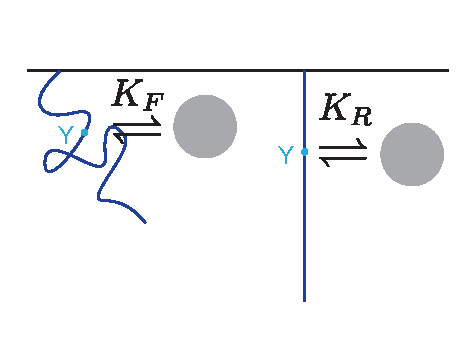
\includegraphics[width=8cm]{figEntropicPenalty.pdf}
%%\caption{ xxxx }
%\label{fig::accuracyFlowchart}
%\end{figure}
%%%%%%%%%%%%%%%%% 
%
%Little is known about the biophysical properties of the zeta-chain (or indeed any unstructured protein domain, which elude crystallography studies). What phosphorylation kinetics are possible? If phosphorylation modifies the polymer properties, e.g., transitions between floppy/unstructured and rigid/structured, can this give rise to cooperativity of phosphorylation and, if so, with what quantitative properties?
%
%
%
%In this project we will perform equilibrium simulations of the zeta-chain interacting with the Lck kinase domain under various assumptions about the effects of phosphorylation. Our aim is to get quantitative estimates and upper bounds for the cooperativity, and other nontrivial kinetics, that can result from the entropic effects of binding to a rigid versus floppy polymer.
%
%
%\textbf{Working title: } Disordered protein domains endow signaling cascades with inherently cooperative kinetics. \textbf{Major question:} What are the ``design advantages" of disordered, polymer domains in signaling? \textbf{Specific question:} What are the cooperativity properties of a multiply-phosphorylated, disordered (floppy) protein that becomes structured (rigid) upon phosphorylation? How does this apply to the T cell signaling cascade, including phosphorylation of the T Cell Receptor zeta-chain by the protein tyrosine kinase Lck? Can this mechanism give rise to high-Hill-number (i.e., ultrasensitive) cooperativity or other nontrivial kinetics? \textbf{Here we: } perform equilibrium calculations of a floppy polymer interacting with a kinase domain under various assumptions about how phosphorylation influences the polymer's structure. We specifically apply results to the TCR zeta-chain and obtain an upper bound on cooperativity in this system. 


%%%%%%%%%%%%%%%%%%%%%%%%%%%%%%%%%%%%%%%%%%%%%%%%%%%
%\section*{Some reading}
%%%%%%%%%%%%%%%%%%%%%%%%%%%%%%%%%%%%%%%%%%%%%%%%%%%
%
%Papers marked with $^{\bullet}$ are of notable interest.
%
%\begin{itemize} 
%\item Background physical chemistry: \citet{Boal:jgXY0Y5Y} \S 3$^{\bullet}$, \citet{Bressloff:RE98Gs4d} \S 1 (free at UCI online)
%\item Reviews: \citet{Wright:2015cw}, \citet{VanDerMerwe:2010hh}, \citet{Brownlie:2013kz}
%\item Primarily theory research papers: \citet{Lenz:2006eo}$^{\bullet}$, \citet{Pontius:1993vu}, \citet{Allard:2012gy}
%\end{itemize}

%%%%%%%%%%%%%%%%%%%%%%%%%%%%%%%%%%%%%%%%%%%%%%%%%%%
\section{Introduction}
%%%%%%%%%%%%%%%%%%%%%%%%%%%%%%%%%%%%%%%%%%%%%%%%%%%

Traditionally, studies of protein function have gone hand-in-hand with studies of protein structure. Proteins such as hemoglobin exhibit complicated behavior, such as cooperativity, by modifying their structure. The cooperative transition of hemoglobin from a closed to open state is well studied with the aid of crystallography and other structure elucidation tools. \hl{CITE} 

Of more recent interest is the behavior of molecules that cannot be crystallized. These proteins lack a defined structure and instead are capable of assuming many different conformations. Although examples of intrinsically disordered proteins (IDPs) have been reported since the 1970s, it was only in the past two decades that they became a focus of major research. \cite{Dunker2008} 

As our understanding of disordered proteins develops, so too will our understanding of a variety of cellular behaviors. These studies will elucidate aspects of signaling, cytoskeleton formation, clustered reactions, and \hl{really.  I need a fourth function.}. Investigations into how disordered proteins mediate each of these processes may lead to new drug targets or introduce new directions for synthetic biology.


%%%%%%%%%%%%%%%%%%%%%%%%%%%%%%%%%%%%%%%%%%%%%%%%%%%
\end{document}
%%%%%%%%%%%%%%%%%%%%%%%%%%%%%%%%%%%%%%%%%%%%%%%%%%%





